\documentclass[twocolumn,oneside,a4paper,12pt]{article}

% ---------------- Para Modificar ---------------- 
\newcommand{\principal}{Volumes}
\newcommand{\conteudo}{}
\newcommand{\turmas}{3~EMSI~A e do 3~EMSI~B}

\date{abril de 2021}

\newcommand{\citacao}{Que nada nos defina. Que nada nos sujeite. Que a liberdade seja a nossa própria substância.}
\newcommand{\autorcitacao}{Simone de Beauvoir}
% ------------------------------------------------

%-------------------------------------------------
\usepackage[english,brazilian]{babel}
\usepackage[alf]{abntex2cite}
\usepackage[utf8]{inputenc}
\usepackage[T1]{fontenc}
\usepackage[top=15mm, bottom=15mm, left=10mm, right=10mm]{geometry}
\usepackage{framed,booktabs,color,hyperref,graphicx}
\usepackage{amsfonts,amsthm,cancel}
\usepackage{subfigure,enumerate,float}
  
\definecolor{shadecolor}{rgb}{0.8,0.8,0.8}
\pagenumbering{arabic}

% Colunas
\usepackage{multicol}
\columnsep=10mm %Espaçamento entre colunas.
\setlength{\columnseprule}{1pt}

% Cabeçalho
\usepackage{fancyhdr}
\pagestyle{fancy}
\lhead{\textbf{\principal}}
\rhead{}
\renewcommand{\headrulewidth}{1pt} % espessura da linha do cabeçalho
\renewcommand{\footrulewidth}{1pt} % espessura da linha do rodapé

% Parágrafo
\setlength{\parindent}{1.25cm}

\newtheorem{problema}{Problema}
\newtheorem{exercicio}{exercicio}
\newtheorem{exemplo}{Exemplo}
\newtheorem{questao}{Questão}

\usepackage[skip=10pt]{caption}
\captionsetup{font={stretch=0.4,small}}

\newcommand{\FRASE}{\textit{``\citacao ''}\\(\textbf{\autorcitacao})}

\title{\LINHAHORIZONTAL \\\textbf{\\ \principal}\footnote{Resumo para os estudos das aulas não presenciais no período de quarentena para as turmas do \turmas .}\\\LINHAHORIZONTAL}

\newcommand{\LINHAHORIZONTAL}{\center \rule{16cm}{1.25pt}}
\newcommand{\sol}{\textbf{Solução}}

\newcommand{\m}[1]{\(\displaystyle {#1}\)}
\newcommand{\M}[1]{\[{#1}\]}

\author{\textbf{Professor Leandro Vieira}\\EREM Regina Pacis\\Palmeirina-PE}
\newcommand{\frase}{\begin{verse} \flushright{\FRASE} \end{verse}}


\begin{document}
\pagestyle{empty}
\cabecalho

\begin{enumerate}
\item Para  disputar  a  final  de  um  torneio  internacional  de natação,  classificaram-se  8  atletas:  3  norte-americanos,  1 australiano,    1    japonês,    1    francês    e    2    brasileiros. Considerando   que   todos   os   atletas   classificados   são ótimos  e  têm  iguais  condições  de  receber  uma  medalha (de  ouro,  prata  ou  bronze),  a  probabilidade  de  que  pelo menos   um   brasileiro   esteja   entre   os   três   primeiros colocados é igual a:
\begin{enumerate}
\item $\frac{5}{4}$
\item $\frac{3}{7}$
\item $\frac{4}{7}$
\item $\frac{9}{14}$
\item $\frac{5}{7}$
\end{enumerate}

\item Em uma urna estão todos os anagramas da palavra CARMA anotados em pedaços de papel idênticos. Tirando um desses papéis ao acaso, qual a probabilidade de que:
\begin{enumerate}
\item As duas letras A do anagrama retirado estejam juntas:
\item As duas letras A do anagrama retirado estejam separadas:
\end{enumerate}

\item Uma um robô vai se deslocar do ponto A até o ponto C da figura a seguir, andando apenas sobre os segmentos de retas mostrados, sempre tomando o menor caminho possível.

	\begin{figure}[!tbh]
	\center
	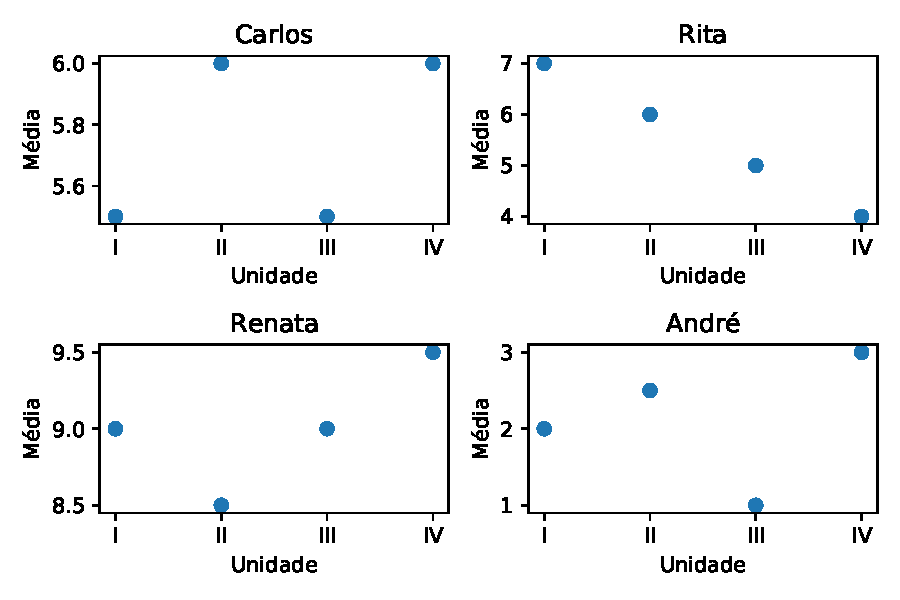
\includegraphics[width=8cm]{01}
	\end{figure}

Sabendo que a maneira como o robô se desloca é aleatória, calcule a probabilidade do robô passar pelo ponto B:

\item seguindo do ponto A ao D na figura, por um caminho de menor comprimento possível, que é feito de maneira aleatória, qual a probabilidade de que o caminho escolhido passe nos pontos B e C:

	\begin{figure}[!tbh]
	\center
	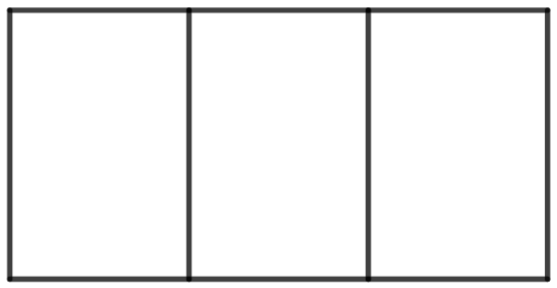
\includegraphics[width=8cm]{02}
	\end{figure}
	
\item Na figura a seguir representa 4 cidades e as estradas entre essas cidades:

	\begin{figure}[!tbh]
	\center
	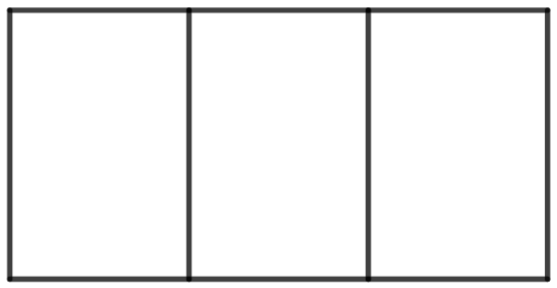
\includegraphics[width=8cm]{02}
	\end{figure}

Sorteando uma dos possíveis trajetos entre as cidades A e D, qual a probabilidade que nesse percurso se passe pela cidade C:

\item  

\end{enumerate}

\FRASE
\end{document}
